% !TeX root = ../../main.tex
\section{Experiments}\label{section:experiments}

Three main experiments were implemented to show how the smartphone can help with common interactions when using \ac{VR} software.
To achieve consistency amongst all experiments in terms of look and functionality, a parent class was implemented. The parent class implements multiple utilities and helpers, which are required by each experiment. It also sets up a basic scene, which contains a sky, a floor and lights.  Also the connection to the \ac{UBII} server is handled. 


\subsection{Model Viewer}\label{subsection:model-viewer}

\acl{VR} offers a new way of experiencing \ac{3D} content. It is more convenient to view a model from different angles and gives a feel of a real presence of the object. Model viewers like Sketchfab\footnote{Sketchfab is an online platform to publish and view 3D content. Website: \href{https://sketchfab.com}{www.sketchfab.com}} have implemented \ac{VR} support a while ago~\cite{Denoyel.2016}. But this experience can be enhanced with a smartphone. Models can be rotated without changing the position of the headset.

\citeauthor{Katzakis.2010} implemented this without \ac{VR}. His approach uses a smartphone to rotate a model, which is displayed on a conventional display. He uses a similar setup, where the phone is wireless connected to a computer, where the model is rendered. The orientation data comes from the magnetometer and, once calibrated to the screen position, is directly mapped to the model~\cite[139]{Katzakis.2010}. In the comparison against a mouse and a touch pen, the smartphone clearly wins in terms of the time it takes to rotate the model to a certain pose~\cite[140]{Katzakis.2010}. 
Since this approach turned out to be very successful, it was used in this experiment as well. 

To feature how easy it is to view a complex model using VR and the smartphone as a manipulator, a skeleton model is used. This experiment is the only one, supporting more than one smartphone client at the moment. For every client that connects, a new skeleton is created. The position is fixed and arranged around the position of the \ac{VR} headset. The scene is shown in Figure~\ref{fig:screenshot-exp-mv}.

\begin{figure}[htpb]
  \centering
  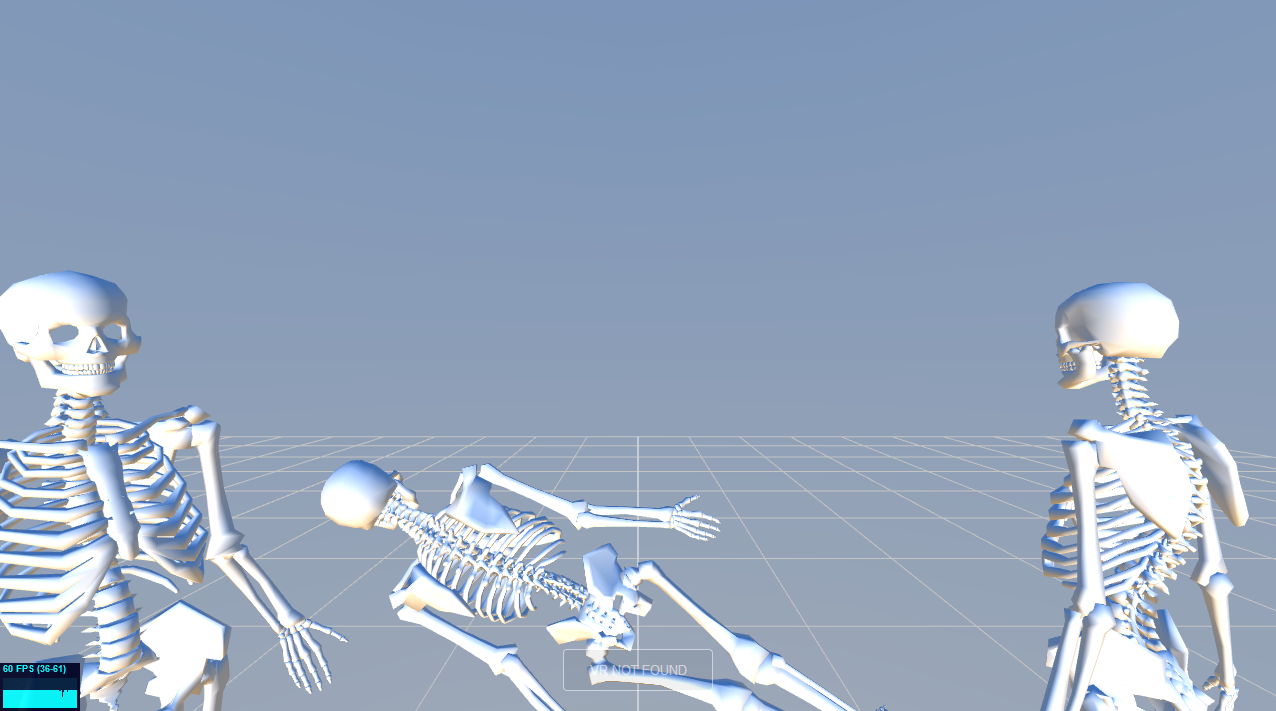
\includegraphics[width=12cm]{figures/screenshot_exp_mv.png}
  \caption[Screenshot: model viewer experiment]{A screenshot of three devices being connected and controlling the rotation of the models.}\label{fig:screenshot-exp-mv}
\end{figure}

% Note: latex thinks the hbox is overfull. This is not the case because something is fixing it. Try removing all words after the lstinline, then you will see that it overflows. But when using in an sentence it appears to be rescaled.
The implementation of this experiment listens for new clients. As soon as one connects, a new interaction is published and the resulting topic is subscribed. Since the smart device publishes the orientation data in a different format than ThreeJS needs for rendering, a reusable interaction was created. The interaction converts the angles from radian to degrees, changes the coordinate system and publishes them to the \lstinline[breaklines=false]{[client id]/SAVRLaserPointer/orientation}-topic. The code for the interaction is shown in Figure~\ref{fig:ubii-interaction-angles}.

\begin{figure}[H]
  \begin{lstlisting}[language=JavaScript]
    function (input, output, state) {
      if (!input) {
        return;
      }

      const deg2Rad = function(v) {
        return v * Math.PI / 180;
      };

      output.orientation = {
        x: deg2Rad(input.orientation.y),
        y: deg2Rad(input.orientation.x),
        z: deg2Rad(-input.orientation.z)
      };
    }
  \end{lstlisting}
  \caption[UBII interaction converting euler angles in radians to degrees]{This interaction is used to convert the orientation data sent by the smart device to the format ThreeJS needs for rendering. The values are converted by multiplying with an approximate of the number $\Pi$ (\enquote{PI}) and dividing by $180$.}\label{fig:ubii-interaction-angles}
\end{figure}


\subsection{Laser Pointer}\label{subsection:laser-pointer}

Selecting elements in a virtual world is a basic interaction most \ac{VR} applications use. The selection of elements in a \ac{2D} environment with standard input devices like a mouse or touch screen is trivial. But the selection of elements in a \ac{3D} environment is problematic, because the element might be too far away from the the user or the cursor. Ray casting\footnote{Ray casting describes a technique to determine the objects which intersect with a ray, cast from a given point into a given direction.} is used to solve this problem: A ray, with the tracked device as origin, is created. Then, the element first hit by the ray is selected. Implementations without a tracked device, often use the position and orientation of the headset. The ray is fixed to the head of the user and casted along his viewing direction~\cite[23]{Kamm.2018}. This forces the user to keep the head still and look at a certain object to select it, until a button is pressed or a certain time has passed.

A better solution is the use of handheld controllers, where the position of the controller is used as origin for the ray. Since the smartphone provides orientation data, it can be used for this task, too. But most handheld controllers have also positional tracking, which allows them to represent the hand of a user by displaying a virtual phone. This emulates the use of a laser pointer in the real world. Since a smartphone does not have positional tracking, the origin has to be somewhere else. Again, the head could be used, but then the user would have no visual representation of the rotation of the phone. To give the user a better feel for direction he is pointing, a visual representation is needed. The user has to see where the ray is going, even when rotating it in the opposite direction of the view direction.

\citeauthor{Argelaguet.2013} evaluated more than 30 different object selection techniques for virtual environments, but there are no technique that uses the orientation but not the position of the pointing device~\cite[Table 1]{Argelaguet.2013}. To work around the missing position data of the device, the ray origin is set to a fixed location relative to the users head where the phone could be in the real world. The ray origin is represented by a \ac{3D} phone model, which orientation is synchronized with the one from the last connected smart device client, similar to the first experiment (\ref{subsection:model-viewer}). To keep the virtual phone inside the view frustum of the user, it rotates relative to the user on the \(y\)-axis.
A line is attached to the front of the phone (the \enquote{laser}) to indicate the direction of the ray.

\begin{figure}[htpb]
  \centering
  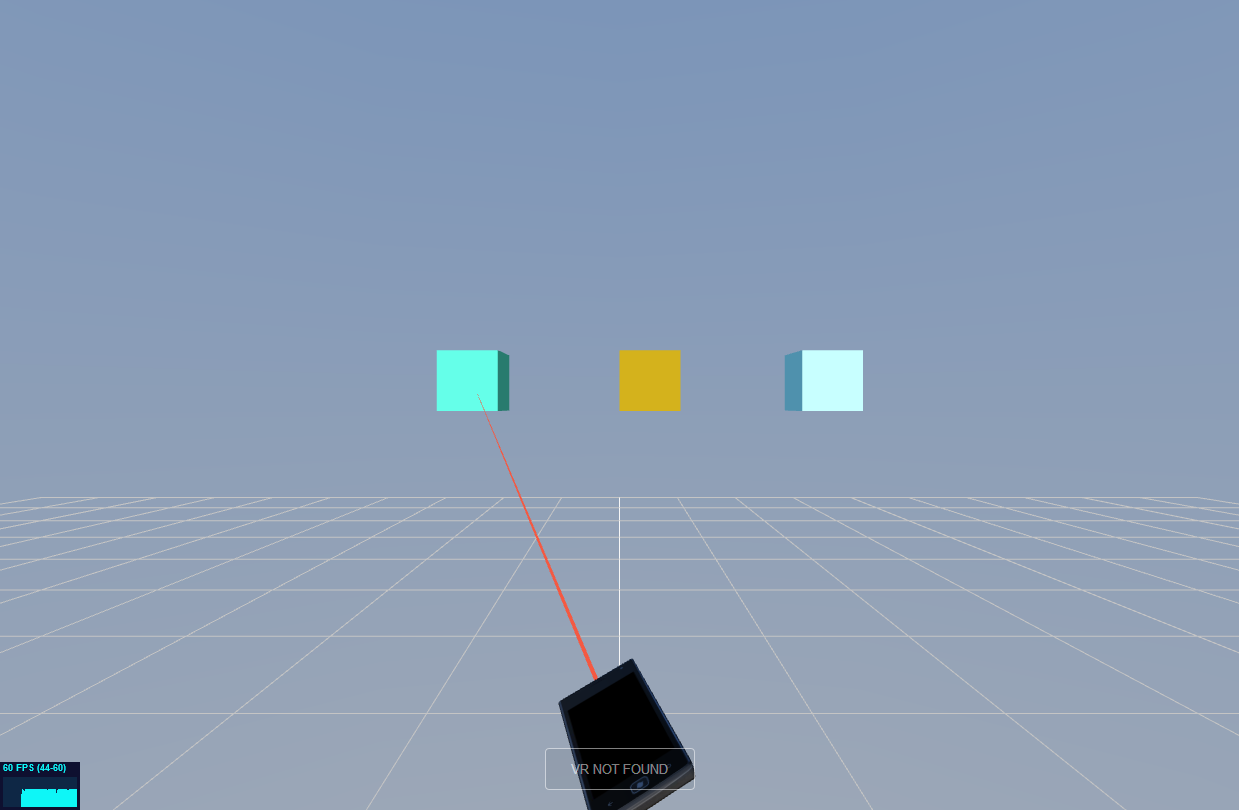
\includegraphics[width=12cm]{figures/screenshot_exp_lp.png}
  \caption[Screenshot: laser pointer experiment]{A screenshot of the virtual laser pointer and selectable cubes.}\label{fig:screenshot-exp-lp}
\end{figure}

In addition to the orientation topic, this implementation subscribes to the touch events topic. The button down event is needed to trigger the actual selection.
In this experiment cubes float in front of the user. If he points the laser at one and touches the display, the cube will change it's color. This works not only with cubes, but with any mesh. Also the system can trigger any kind of event or action. A screenshot of this setup can be seen in Figure~\ref{fig:screenshot-exp-lp}.


\subsection{Virtual Keyboard}\label{subsection:virtual-keyboard}

text input is difficult task to solve
es gibt speech input und input mit motion controllern wo man buttons einer tastatur drift..

auch gut\dots




\begin{figure}[htpb]
  \centering
  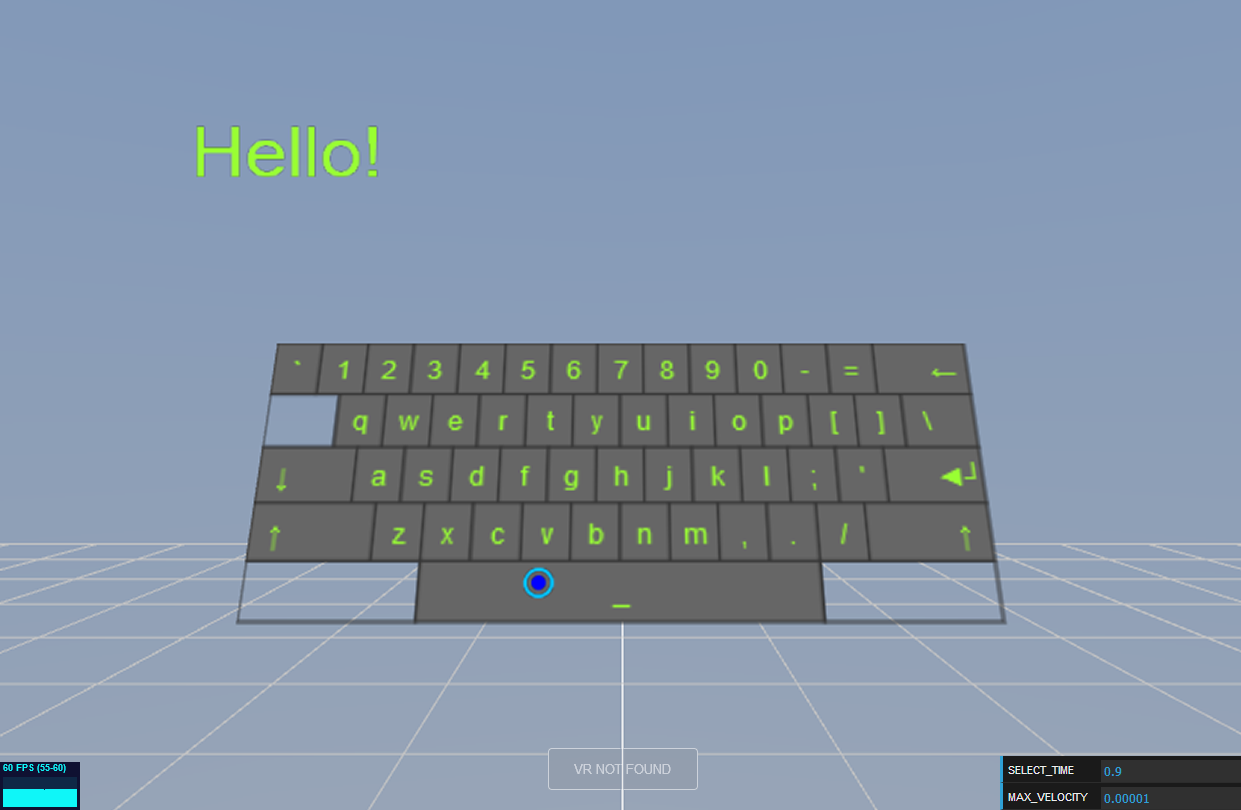
\includegraphics[width=12cm]{figures/screenshot_exp_vk.png}
  \caption[Screenshot: virtual keyboard experiment]{A screenshot of the virtual keyboard with the blue cursor and the previously typed text.}\label{fig:screenshot-exp-vk}
\end{figure}
